\section{Theoretische Grundlagen}
\subsection{Biometrie}
\subsectionauthor{Torben Brenner}
Bei der Biometrie handelt es sich um eine Wissenschaft, welche sich mit der Vermessung von biologischen Merkmalen beschäftigt.\newline
Die Ergebnisse dieser Messungen können dann dazu verwendet werden, Individuen zu beschreiben und zu identifizieren. Dieser Bereich 
der Biometrie wird auch als \textit{biometrische Erkennungsverfahren} beschrieben. Eine andere Facette der Biometrie, die \textit{biometrische Statistik},
beschäftigt sich mit der Auswertung der erfassten Daten um diese zur Analyse zu nutzen.\newline
Mit der biometrischen Statistik, werden wir uns in dieser Studienarbeit beschäftigen, um die Merkmale, die mittels 
Smartphone erfasst werden, auszuwerten und damit Rückschlüsse auf die Emotionen eines Menschen zu ermöglichen.
\subsection{Smartphone}
\subsectionauthor{Torben Brenner}
Ein Smartphone differenziert sich durch mehrere Aspekte von einem herkömmlichen Telefon. Der erste Unterschied, so wie alten mobil Telefonen, ist das Telefonieren ohne direkten Kabelanschluss an das Netz oder zusätzliche Basisstation.\newline 
Wodurch es sich aber von den eben genannten mobil Telefonen unterscheidet, ist die Leistungsfähigkeit der einzelnen Komponenten. So besitzen heutige Smartphones häufig Prozessoren mit Acht Kernen und Leistungen ab 1,7 GHz pro Kern. Neben der Leistungsfähigkeit des Prozessors ist auch die Menge des verbauten Hauptspeichers gewachsen. Die wenigsten Smartphones besitzen heute noch weniger als 2 Gigabyte Arbeitsspeicher. Diese stärkeren Komponenten ermöglichen das ausführen komplexer Anwendungen und außerdem Multitasking. Das lässt beim Vergleich mit der Definiton eines Computers es auch zu, zu behaupten das Smartphones ebenfalls Computer sind. \textbf{TODO: das hier mit quellen und bezug auf die beiden definitionen}\newline
Der Hauptunterschied ist aber die Menge der verbauten Sensoren. Wie Kai Biermann auf Zeit Online schreibt, ermöglichen diese es einem Smartphone zu sehen, fühlen und hören \footcite[Vgl.][S. 1 Abs. 2]{Bie14}. In diesem Artikel beschreibt Biermann die enormen Möglichkeiten die diese Sensoren ermöglichen. So ermöglicht ein Smartphone die Navigation per Positionsbestimmung, das Mikrofon das hören und die Handykamera ermöglicht dem Smartphone das sehen. Gerade weil Smartphone Kameras immer besser werden sind die Möglichkeiten zur Gesichtserkennung deutlich gestiegen, wie zuletzt Apple mit dem IPhone X zeigte, das Emotionen über die Kamera erkennt und diese auf die sogenannten Animojis überträgt. \textbf{TODO: Finde Quelle für diese Aussage} 
\subsection{Was sind Emotionen?}
\subsectionauthor{Torben Brenner}
Da wir uns in dieser Arbeit primär mit der Erkennung von Emotionen beschäftigen wollen, ist es wichtig den Begriff Emotion zu definieren.
Schwarzer-Petruck beschreibt in ihrem Werk Emotionen und pädagogische Professionalität eine Emotion als \textit{``ein komplexes
Muster körperlicher und mentaler Veränderungen als Antwort auf eine als persönlich bedeutsam wahrgenommene Situation''}\footcite[S.51 Z.20ff]{Sch13}.
Das Muster umfasst laut Schwarzer-Petruck die Aspekte des kognitiven Prozess, die Gefühle, eine Verhaltensreaktion und eine physiologische Erregung.
\subsection{Grundlagen der Emotionserkennung}
\subsectionauthor{Torben Brenner}
Nach dem nun geklärt ist was unter einer Emotion verstanden wird, stellt sich die Frage wie man diese erkennen kann. Das Problem hierbei ist, dass es eine große Anzahl an Emotionen gibt, laut Hokuma\footcite[Vgl.][Absch. 1]{Hok17} sind es 34.000 unterschiedliche Emotionen. Diese verschiedenen Emotionen lassen sich nur schwer erfassen und unterscheiden, weshalb ein Weg gefunden werden muss die Emotionen einzuteilen. Diese Einteilung wurde bereits von Robert Plutchick vorgenommen und herausgekommen sind dabei acht primäre Emotionen: Freude, Traurigkeit, Akzeptanz, Ekel, Angst, Wut, Überraschung und Erwartung.\newline
Mit diesen acht Emotionen hat Plutchick das Rad der Emotionen gebildet(siehe Abbildung).
\begin{figure}[h]
	\centering
	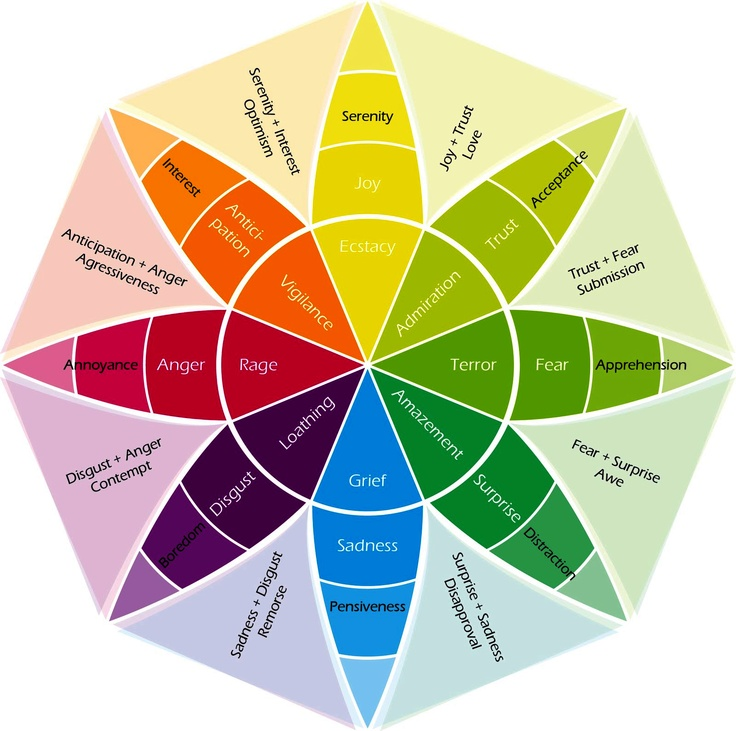
\includegraphics[width=16cm]{Bilder/wheel-of-emotions.png}
	\caption[Rad der Emotionen - Robert Plutchick]{Rad der Emotionen - Robert Plutchick\footnotemark}
\end{figure}%
\footcitetext[Vgl.][]{Hok17}
\newline
Das Rad stellt die primären Emotionen dabei in Relation, wobei die Kombinationen zwischen zwei Emotionen im Raum zwischen diesen steht und Emotionen die gegensätzlich wirken, z. Bsp. Traurigkeit und Freude, jeweils auch gegenüberliegend auf dem Rad sind. Außerdem wird die Stärke einer Emotion durch deren nähe zum Zentrum des Rads gekennzeichnet, z. Bsp. Wut zu toben \footcite[Vgl.][Absch. Elements of the Wheel]{Hok17}.\newline
In der Literatur gibt es neben dem Model von Plutchick auch das \textit{Gevena Emotion Wheel}. Dieses Modell betrachtet die Emotionen nicht in acht primären Hauptkategorien, sondern unterscheidet zwischen 20 Emotionen anhand von zwei Parametern, die Valenz und die Kontrolle. Die Kontrolle bezeichnet, wie stark Individuum eine Situation kontrollieren kann. Die Valenz sagt aus ob eine Situation für das Individuum eher angenehm oder unangenehm ist.\newline 
Beide Modelle können dafür genutzt werden um Emotionen auszuwerten, wobei hier zu diskutieren ist welches Modell besser geeignet ist.
\subsection{Umgang mit biometrischen Daten}
\subsectionauthor{Torben Brenner}
Eine Problematik, mit der wir uns in dieser Arbeit beschäftigen müssen, ist der Umstand das biometrische Daten nicht immer einen direkten Schluss auf einen Emotion zulassen. So lässt ein hochfrequenter Puls keinen direkten Schluss auf die Emotion zu die ein Individuum gerade empfindet. Er kann maximal ein Indiz für verschiedene Emotionen sein, z. Bsp. Wut oder Angst. Um mit diesem Umstand umzugehen benötigen wir zwei neue Begriffe die im folgenden genauer erläutert werden. 
\subsubsection{Indiz}
Ein Indiz ist im allgemeinen Sprachgebrauch ein Anzeichen für einen Umstand, an dem sich ein Zustand oder eine Entwicklung absehen lässt\footcite[Vgl.][]{Dud18}. In unserer Arbeit, sehen wir Daten die wir von den Sensoren bekommen, als Indizien an. Ein Indiz macht es wahrscheinlicher bzw. unwahrscheinlicher das ein Individuum eine bestimmte Emotion verspürt. 
\subsubsection{Kausalität}
Als Kausalität wird im allgemeinen der Zusammenhang zwischen Ursache und Wirkung verstanden. In der Physik ist die Kausalität ein grundlegendes Prinzip, welches besagt, ``daß in der Natur nichts ohne Grund passiert, d.h. zu jedem Ereignis (Wirkung) ein anderes (Ursache) existiert, das a) in seiner Vergangenheit liegt und b) zwingende Voraussetzung für das Eintreten der Wirkung ist''\footcite{Sav18}.\newline
In dieser Arbeit werden wir ebenfalls versuchen, kausale Zusammenhänge zwischen Reaktionen des Körpers und den gerade empfundenen Emotionen zu ermitteln.
Ein Werkzeug um kausale Zusammenhänge darzustellen ist in der Literatur der Kausale Graph (im englischen \textit{directed acyclic graph}).
\begin{figure}[h]
	\centering
	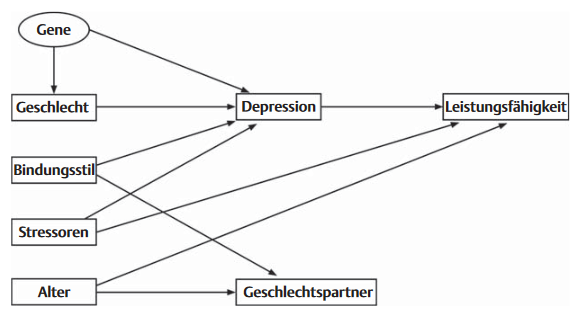
\includegraphics[width=11cm]{Bilder/dag.png}
	\caption[Fiktives Beispiel eines DAGs]{Fiktives Beispiel eines DAGs\footnotemark}
\end{figure}
\footcite[Vgl.][Kausale Graphen - DAGs]{Tho11}
Die Grafik zeigt ein fiktives Beispiel für einen kausalen Graphen. In diesem Beispiel von Thoemmes wird dargestellt das Bindungsstil, Geschlecht, Stressoren und Gene Einfluss auf Depressionen haben. Wichtig ist, dass alle Annahmen die in einem solchen Graph gemacht werden theoretisch begründet werden müssen. Ist dies nicht der Fall, dürfen sie kritisiert und infrage gestellt werden \footcite[Vgl. ][S.3 Kausale Graphen - DAGs]{Tho11}.
\subsection{Emotionsindizien}
\subsubsection{Puls}
\subsubsection{Hautleitfähigkeit/Hautwiderstand}
\subsubsectionauthor{Lukas Seemann}
Die menschliche Haut verfügt über \glqq \textit{aktive als auch passive elektrische Eigenschaften, die sich auf Strukturen und Fuktionen der Haut und der in ihr enthaltenen Organe zurückführen lässt.}\grqq{}\footcite[][S. 2]{Bou88} Diese elektrischen Phänomene der Haut sind in wissenschaftlichen Kreisen unter dem Sammelbegriff elektrodermale Aktivität (kurz EDA) bekannt. \footcite[Vgl.][S. 2]{Bou88}
Eine elektrodermale Aktivität, die sich sehr gut als Indikator für Emotionen eignet, ist die Hautleitfähigkeit. Hierzu wird mit einer externen Stromquelle mit geringer Spannung gemessen, wie gut die Haut eines Probanden diesen Strom leitet. \footcite[Vgl. ][S.77]{Moe07} Häufig wird anstand der Hautleitfähigkeit auch der Hautwiderstand gemessen. Diese beiden Indizien stehen in einer negativ proportionalen Beziehung. Dies bedeutet, je höher der Widerstand der Haut ist, desto niedriger ist die Leitfähigkeit und umgekehrt. Letzten Endes sagen beide Indizien dasselbe aus, unterscheiden sich aber in der Betrachtungsrichtung. \footcite[Vgl. ][S. 28]{Die06} \newline
Die Hautleitfähigkeit wird anhand der Menge von Schweiß an den Ausgängen der Schweißdrüßen bestimmt, die sich über den gesamten Körper veteilen. Je mehr Schweiß, der elektrisch sehr gut leitend ist, sich auf der Haut befindet, umso größer ist die Hautleitfähigkeit. Am besten eignen sich  Stellen, an denen die Schweißdrüsen sehr dicht angeordnet sind und die somit sehr schweißsensibel sind. Dies ist zum Beispiel an den Handinnenflächen beziehungsweise Fingerinnenseiten der Fall, die sich deshalb sehr gut für solche Messungen eignen. \footcite[Vgl. ][S.77]{Moe07} 
\begin{figure}[h]
	\centering
	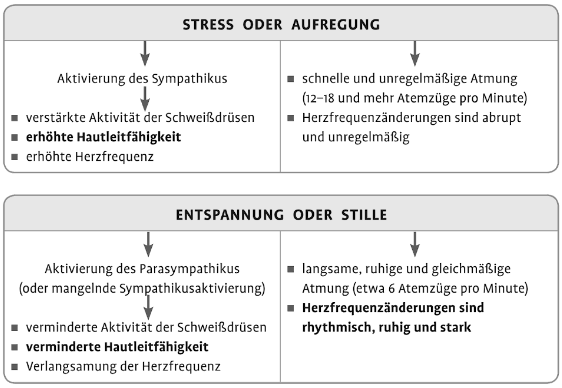
\includegraphics[width=14.6cm]{Bilder/symp.png}
	\caption[Reaktion des Körpers auf Stress und Entspannung]{Reaktion des Körpers auf Stress und Entspannung\footnotemark}
\end{figure}%
\footcitetext[][S. 200]{Dil13}
\newline
\glqq \textit{Die Aktivation beschreibt das Ausmaß der physiologischen Aktiviertheit oder Wachheit eines Menschen}\grqq{}\footcite[][S. 28]{Die06}. Unter Aktivitation versteht man bei Menschen generell jede Art von emotionaler Erregung. Hierzu zählen unter anderem Wut, Aufregung, Schreckmomente oder auch extreme Freude. In Abbildung 3 ist die Reaktion des Körpers auf Stress (darausfolgend auch Aktivation) und auf Entspannung dargestellt. Die Schweißprodukation wird über das unwillkürliche Nervensystem gesteuert. Dieses besteht aus Sympathikus der für die Bereitstellung von Energie und Arbeitsleistungs zustöndig ist, und dem Parasympathikus, der zur Erholung und Wiederherstellung von Körperfunktionen dient. \footcite[Vgl. ][S. 5]{Lie13} \newline Bei Stress oder Aufregung wird der Sympathikus aktiviert, was eine versträkt Schweißproduktion und somit auch eine erhöhte Hautleitfähigkeit hervorruft. Außerdem wird die Herz- und Atemfrequenz erhöht und der Rhymtmus dieser ist unregelmäßig. Die Reaktion auf ein Ereignis, das emotionale Erregung hervorruft, lässt sich meistens innerhalb von einer bis vier Sekunden anhand der Änderung der Hautleitfähigkeit feststellen. \footcite[Vgl.][S. 130f]{Sch14} \newline 
Bei Entspannung hingegen wird der Parasympathikus aktiviert, was zu einer verminderten Aktivität der Schweißdrüßen führt. Die Hautleitfähigkeit sinkt somit auch. Des Weiteren werden Herz- und Atem verlangsamt und gelangen wieder in einen normalen Rhymthmus. \newline
Der Vorteil der Messung der Hautleitfähigkeit ist, dass diese unwillkürlich gesteutert wird und somit keine willentliche Mitarbeit des Probanden erfodert. Da die Aktivierung des Sympathikus automatisch geschieht, kann der Proband die Messung nicht verfälschen. \newline
Ein Nachteil des Verfahren ist, dass die Hautleitfähigkeit nur Rückschlüsse auf den Grad der Aktiviation schließen lässt, jedoch nicht gesagt werden kann, ob es sich um positive oder negative Reaktionen handelt. Die Wut über ein Ereignis würde zum selben Ergebnis führen, wie die übermäßige Freude über ein Ereignis. Aus diesem Grund müssen zur genauen Emotionsbestimmung weitere Indizien herangezogen werden. \footcite[Vgl. ][S.77]{Moe07}

\subsubsection{Gesichtszüge}
\subsubsection{Tippverhalten}
\subsection{Erfassungsmöglichkeiten des Smartphones}
\subsubsection{Nutzerinteraktionen}
\subsubsectionauthor{Torben Brenner}
Im Laufe des Alltags verwenden Nutzer ihr Smartphone sehr häufig. Dabei können unteranderem Aspekte wie das Tippverhalte, 
z. Bsp. verwendet der User viele Smileys, Rückschlüsse auf den emotionalen Zustand eines Nutzers ermöglichen.
\subsubsection{Im Smartphone eingebaute Sensoren}
\subsubsection{Zusätzliche Hardware}
Im Rahmen des Projektes wird die Möglichkeit erforscht, mit Hilfe eines Arduinos die Hautleitfähigkeit aufzuzeichnen. 
Diese ist ein großer Faktor bei der Bestimmung von Emotionen und wird unteranderem auch in Lügendetektoren verwendet. 
\begin{figure}[h]
	\centering
	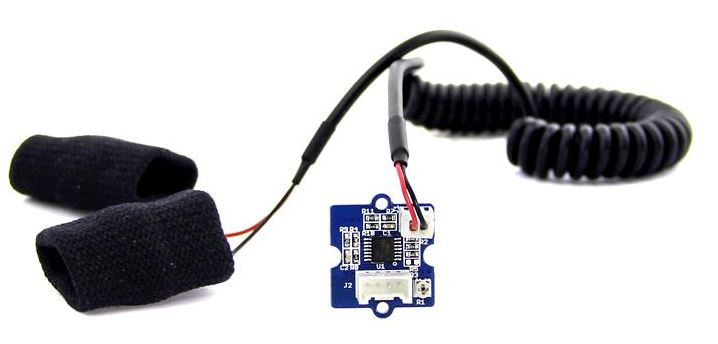
\includegraphics[width=11cm]{Bilder/sensor.jpg}
	\caption{Das ist ein cooler GSR Sensor}
\end{figure}%